\documentclass[12pt]{article}

\usepackage{answers}
\usepackage{setspace}
\usepackage{graphicx}
\usepackage{enumitem}
\usepackage{multicol}
\usepackage{mathrsfs}
\usepackage[margin=1in]{geometry} 
\usepackage{amsmath,amsthm,amssymb}
\usepackage[ngerman]{babel}

\newcommand{\N}{\mathbb{N}}
\newcommand{\Z}{\mathbb{Z}}
\newcommand{\C}{\mathbb{C}}
\newcommand{\R}{\mathbb{R}}

\DeclareMathOperator{\sech}{sech}
\DeclareMathOperator{\csch}{csch}

\newenvironment{theorem}[2][Theorem]{\begin{trivlist}
		\item[\hskip \labelsep {\bfseries #1}\hskip \labelsep {\bfseries #2.}]}{\end{trivlist}}
\newenvironment{definition}[2][Definition]{\begin{trivlist}
		\item[\hskip \labelsep {\bfseries #1}\hskip \labelsep {\bfseries #2.}]}{\end{trivlist}}
\newenvironment{proposition}[2][Proposition]{\begin{trivlist}
		\item[\hskip \labelsep {\bfseries #1}\hskip \labelsep {\bfseries #2.}]}{\end{trivlist}}
\newenvironment{lemma}[2][Lemma]{\begin{trivlist}
		\item[\hskip \labelsep {\bfseries #1}\hskip \labelsep {\bfseries #2.}]}{\end{trivlist}}
\newenvironment{exercise}[2][Exercise]{\begin{trivlist}
		\item[\hskip \labelsep {\bfseries #1}\hskip \labelsep {\bfseries #2.}]}{\end{trivlist}}
\newenvironment{solution}[2][Solution]{\begin{trivlist}
		\item[\hskip \labelsep {\bfseries #1}]}{\end{trivlist}}
\newenvironment{problem}[2][Problem]{\begin{trivlist}
		\item[\hskip \labelsep {\bfseries #1}\hskip \labelsep {\bfseries #2.}]}{\end{trivlist}}
\newenvironment{question}[2][Question]{\begin{trivlist}
		\item[\hskip \labelsep {\bfseries #1}\hskip \labelsep {\bfseries #2.}]}{\end{trivlist}}
\newenvironment{corollary}[2][Corollary]{\begin{trivlist}
		\item[\hskip \labelsep {\bfseries #1}\hskip \labelsep {\bfseries #2.}]}{\end{trivlist}}

\begin{document}
	\title{Programmieren mit Neuronalen Netzen}
	\author{Michael Gabler}
	\maketitle
	\tableofcontents
	\newpage

	\section{Grundlagen}
	Neuronales Netzwerk ist Funktion, die auf Eingabedaten angewendet wird.\\
	\textbf{Optimierung} durch Minimierung der Loss-Funktion\\
	\textbf{Loss-Funktion} Maß, wie gut das Netzwerk Vorhersagen trifft. Berechnet sich aus Vorhersage und tatsächlichen Werten (Ground Truth).
	\begin{itemize}
		\item Euklidischer Loss, Mean-Squared-Error: $l_2 = \frac{1}{2N} \sum_i (f_\theta(x_i)-t_i)^2$
		\item Negative-Log-Likelihood, Cross-Entropy: $NLL = -\frac{1}{|D|}\sum_i \log[f_\theta(x_i)|_{t_i}]$
		
	\end{itemize}
	
	\subsection{Training}
	Daten werden aufgeteilt in Train/Validierung/Test (z.B. 60/20/20)\\
	\textbf{Epoche} Verarbeitung aller Trainingsdaten\\
	\textbf{Iteration} Verarbeitung eines Batches\\
	\textbf{Batch} Mehrere Trainingsbeispiele werden gerechnet bevor Gewichte einmal geupdated werden (z.B. 10 Beispiele pro Batch)\\
	\textbf{Evaluation auf Validierungsdaten} zur Anpassung der Hyperparameter (Learning-Rate, Netzstruktur, ...)\\
	\textbf{Evaluation auf Testdaten} einmalig, um Genauigkeit des trainierten Netzes zu ermitteln
	\textbf{Forward-Pass} Berechnen des Outputs des Netzwerkes für bestimmte Eingabedaten (z.B. ein Batch)\\
	\textbf{Backward-Pass} Bilden der partiellen Ableitung für jeden Input in jedem Layer und Speichern der Werte als Deltas\\
	\textbf{Berechnung der Gewicht-Deltas}\\
	\textbf{Update der Gewichte}

	\subsection{Netzarchitektur}
	\textbf{Perceptron} (= künstliches Neuron) stellt lineare Trennung (binäre Klassifikation) dar. Kann Funktionen AND, OR und NOT lernen, nicht aber XOR.\\
	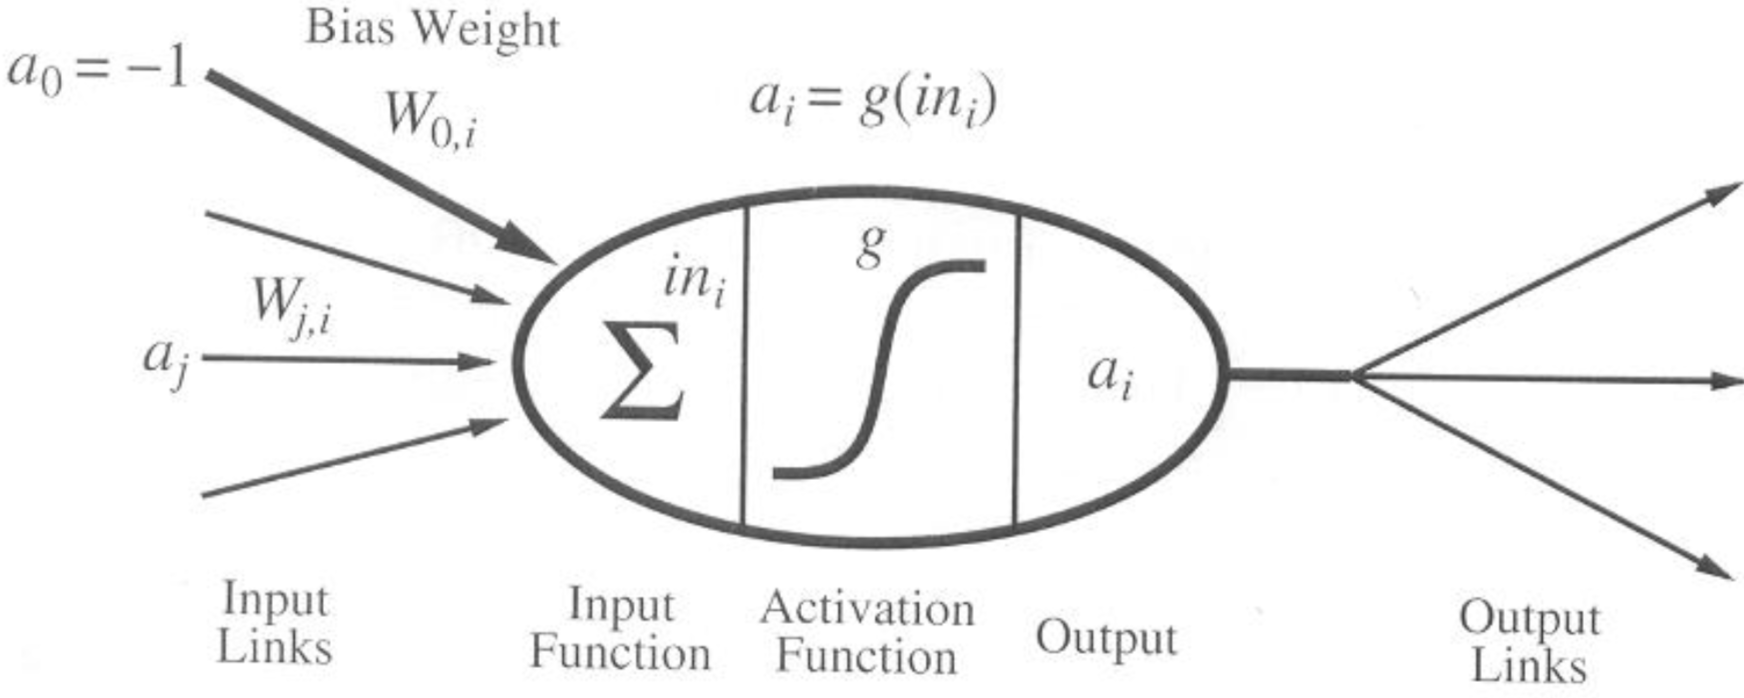
\includegraphics[width=\linewidth]{figures/perceptron.png}\\
	mit Inputs $a_j$ gewichtet mit $W_{ji}$ (ergeben zusammen die Gewichtsmatrix $W$), addiert mit Bias $b$, Outputs $a_i$ und der Aktivierungsfunktion $g$ mit der der Output berechnet wird.
	$$Ausgabe_{Schicht(x)} = g(Eingabe_{Schicht(x)} \cdot W + b) = Eingabe_{Schicht(x+1)}$$
	\textbf{Aktivierungsfunktion} muss bei Multi-Layer-Perceptronen (MLP) nicht-linear sein, da sonst nicht mehr Information gespeichert werden kann.
	$$(x \cdot W + b) \cdot V + a = x \cdot W \cdot V + b \cdot V + a = x \cdot W' + b'$$

	\section{Layer}
	Mögliche Schichten aus denen ein neuronales Netz bestehen kann.
	\subsection{Fully Connected}
	\subsection{Aktivierungsfunktion}
	Aktivierungsfunktionen mit Ableitungen
	\subsection{Softmax}
	\subsection{Dropout}
	Für Regularisierung verwendet
	\subsection{Convolutional}
	\subsection{Pooling}
	\subsection{Vanilla RNN}
	\subsection{LSTM}
	\subsection{Gru}



	\section{aus alter Vorlesung}
	\textbf{Perceptron} (= künstliches Neuron) stellt lineare Trennung (binäre Klassifikation) dar. Kann Funktionen AND, OR und NOT lernen, nicht aber XOR.\\
	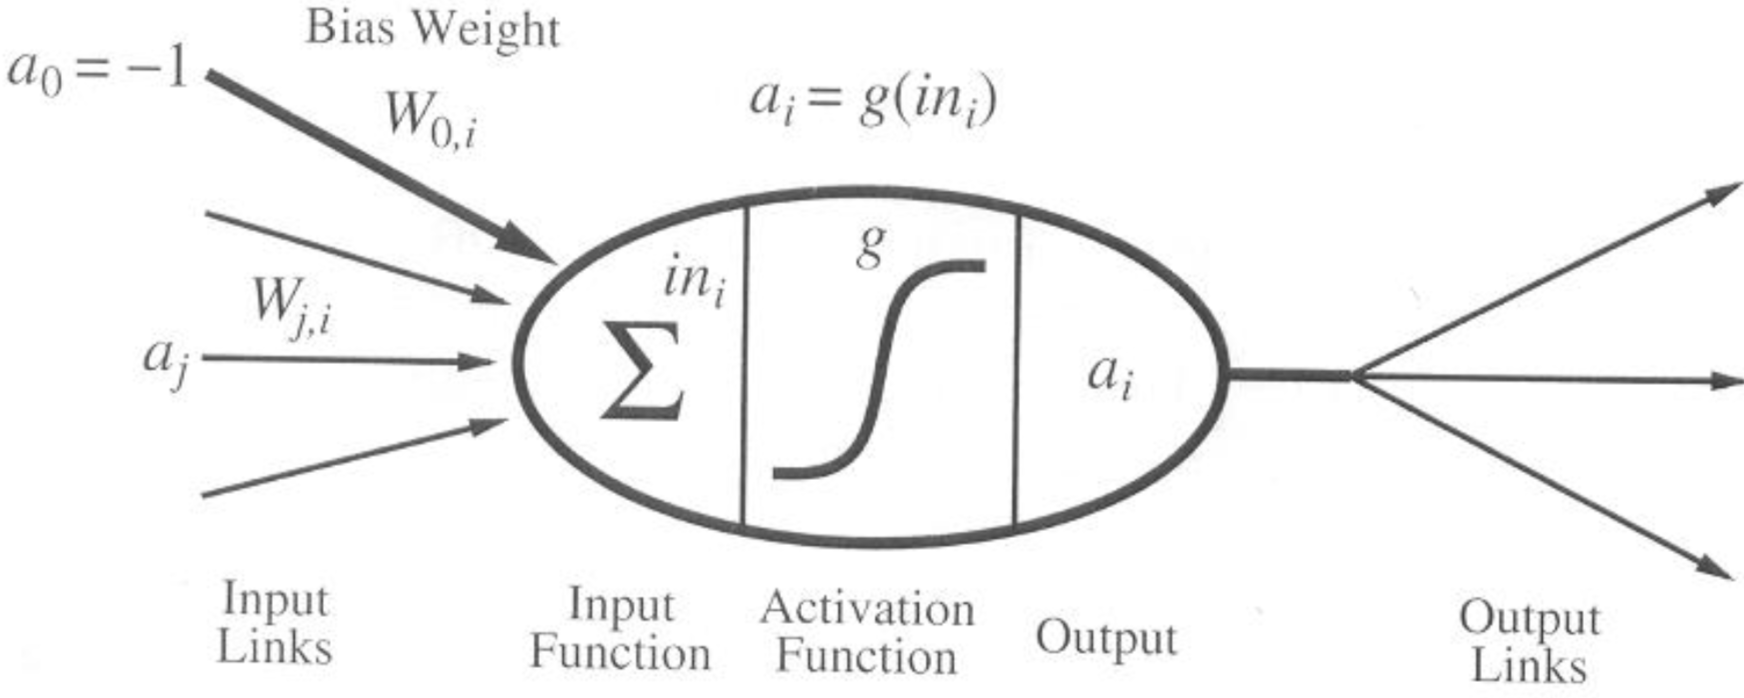
\includegraphics[width=\linewidth]{figures/perceptron.png}\\
	mit Inputs $a_j$ gewichtet mit $W_{ji}$ (ergeben zusammen die Gewichtsmatrix $W$), Outputs $a_i$ und der Aktivierungsfunktion $g$ mit der der Output berechnet wird.\\
	\textbf{Bias} ist der Input eines Perceptrons, der immer konstant bleibt (meist 1) damit das Perceptron auch bei schwachem Input nicht abgeschaltet wird.\\
	\textbf{Aktivierungsfunktionen} typisch sind:
	\begin{itemize}
		\item Stufenfunktion: $g(x) = x < 0 \rightarrow 0, x > 0 \rightarrow 1$ (nicht differenzierbar)
		\item Sigmoidfunktion: $g(x) = \frac{1}{1 + e^{-x}}$ (siehe Einleitung Lernen)
		\item ReLU (Rectified Linear Unit): $g(x) = x < 0 \rightarrow 0, x > 0 \rightarrow x$ (nicht differenzierbar für $x=0$)
		\item Tangenz hyperbolicus: $g(x) = tanh(x)$
		\item Softmax: Abbildung eines Vektors in Werte zwischen 0 und 1 mit Summe 1 (z.B. für Ausgabelayer)
	\end{itemize}
	\textbf{Loss-Funktion} Liefert einen Wert, der repräsentiert, wie gut ein neuronales Netz bereits trainiert ist. Wird anhand des Abgleichs von Vorhersage und tatsächlichem Wert (Ground Truth) berechnet.\\
	\textbf{Berechnung der Ausgabe}
	$$Ausgabe_{Schicht(x)} = g(W \cdot Eingabe_{Schicht(x)}) = Eingabe_{Schicht(x+1)}$$
	\textbf{Rückpropagierung} Fehler (z.B. quadratische Abweichung von erwartetem Wert $\rightarrow$ Loss-Funktion) wird entsprechend der Gewichte auf Vorgängerknoten verteilt\\
	\textbf{Verteilung des Fehlers}
	$$Fehler_{Schicht(x-1)} = W^T \cdot Fehler_{Schicht(x)}$$
	Änderung der Gewichte über Gradient Descent $w_{jk} \leftarrow w_{jk} - \alpha \frac{dE}{dw_{jk}}$ mit $E$ als Loss-Funktion\\
	\textbf{Datenvorverarbeitung} Inputs zwischen 0 und 1, da hohe Werte niedrige Gradienten erzeugen, Bilder können rotiert, gespiegelt, zugeschnitten, etc. werden um mehr Trainingsdaten zu generieren.\\
	\textbf{Netzvorbereitung} zufällige Vorbelegung der Gewichte (nicht symmetrisch) $\Rightarrow$ Pre-Training: wenn möglich Gewichte eines bereits trainierten Netzes für ähnliches Problem verwenden\\
	\textbf{Overfitting} kann durch kleine Netzgröße (nicht so ausdrucksstark), Dropout (ignorieren einiger Knoten für einen Lerndurchgang)\\
	\textbf{Typen von Schichten}
	\begin{itemize}
		\item Fully Connected (FC): besteht aus mehreren Perceptrons (s.o.)
		\item Convolutional Neural Networks (CNN): Für Bilderkennung, Gewichtungsmatrix über Input verschieben und gewichtete, aufsummierte Werte in Outputmatrix schreiben
		\item Polling Layer: Verkleinerung von Inputmatrizen durch z.B. Max-Funktion einer Submatrix
	\end{itemize}
	\textbf{Multi-Klassen Klassifizierung} über $K$ Diskrimianzfunktionen für $K$ Klassen. Dabei gibt immer eine Funktion für einen bestimmten Bereich/Klasse den höchsten Wert zurück.\\
	\textbf{Vanishing Problem} Tiefe Netze lernen sehr langsam, da das Änderungsgewicht pro Schicht mit Faktor < 1 multipliziert wird (Ableitung Aktivierungsfunktion). Kann umgangen werden durch ReLU (Ableitung konstant 1 für positive Zahlen)\\
	\textbf{Recurrent Neural Networks} für die Verarbeitung von sequenziellen Daten (variable Ein-/Ausgabe) z.B. für OCR oder Sprachverarbeitung\\
	\textbf{Adversial Examples} Manipulierte Inputdaten, die für den Menschen noch gut erkennbar sind (kein merklicher Unterschied zu Original), von einem DNN jedoch falsch klassifiziert werden. Bild wird mit Rauschen addiert, welches auf das Netz trainiert ist. Gegenmaßnahmen:
	\begin{itemize}
		\item Trainiere Netz mit Adversial Examples (richtige Klassifikation)
		\item Mehrere unterschiedliche Technologien zur Klassifikation einsetzen
		\item DeepCloak entfernen von unnötigen Features, die ausgenutzt werden könnten
	\end{itemize}
	
\end{document}
